\chapter{Case Study - DESIGNING A CAMPGROUND - SIMPLEX METHOD}
\todoChapter{ 0\% complete. \\
Notes: Borrowed from Karin Vorwerk.  Need to integrate this into other chapters.}
\section{DESIGNING A CAMPGROUND - SIMPLEX METHOD}
The Simplex method is probably the classic method of solving constraint optimization problems. We will use this solution approach, sometimes in modified form, over and over in this class, not just in this chapter.

\begin{outcome}
You will learn

\begin{itemize}
  \item How to recognize linear programming (LP) problems

  \item Vocabulary of LP problems

  \item Graphical solution

  \item Algebraic solution

  \item Excel solution with the Excel Solver

\end{itemize}
\end{outcome}
\subsection{Case Study Description - Campground}
You are opening a campground in the Florida Keys, and you are trying to make as much money as possible. You are planning a mix of RV sites, tent sites, and yurts. Let's assume you already own 10 acres, and that you can make $\$ 80 /$ day profit on each $\mathrm{RV}, \$ 20 /$ day profit on each tent, and $\$ 200$ profit on each Yurt. However, there are restrictions:

\begin{enumerate}
  \item Infrastructure takes up $20 \%$ of your site

  \item You can have 20 RVs per acre, or

  \item You can have 40 tents per acre, or

  \item You can have 10 yurts per acre

  \item You have a budget of $\$ 100,000$. It costs you $\$ 1000$ to develop an $R V$ site, $\$ 200$ for a tent site, and $\$ 8000$ for a yurt.

  \item Maintenance for the bath houses etc. is $15 \mathrm{~min} /$ week/camper unit. You can afford 70hrs/week in maintenance help

  \item Zoning ordinance requires you to have at least 20 tent sites What is the best layout for your campground, and how much profit can you make per day?

\end{enumerate}
\subsection{References}
This case study was inspired by the Knights Key RV park in Florida. Read more about it here: \href{http://www.knightskeyrvresortandmarina.com/news/}{http://www.knightskeyrvresortandmarina.com/news/} \href{http://www.miaminewtimes.com/news/developers-plan-to-replace-rv-park-with-fivestar-resort-stirs-fears-hopes-in-keys-8038648}{http://www.miaminewtimes.com/news/developers-plan-to-replace-rv-park-with-fivestar-resort-stirs-fears-hopes-in-keys-8038648}

\subsection{Solution Approach - Two Variables}
We will again first look at a simpler problem by ignoring the yurts and only considering RV spaces and tents.

Let $r$ be the number of RVs, $t$ the number of tents, and $P(r, t)$ the profit. Your goal is to maximize $P(r, t)=$ $80 \mathrm{r}+20 \mathrm{t}$. This function is called the objective function. The variables $r$ and $t$ are called decision

variables. You can see that in the current case $P(r, t)$ gets bigger if you increase $r$ and/or $t$. If you picture a graph with $r$ on the horizontal and $t$ on the vertical axis, then the direction of increase for the objective function is to the top right.

Translating the relevant restrictions into equations gives

\begin{enumerate}
  \item $r / 20+t / 40 \leq 8$

  \item $r \leq 160$

  \item $t \leq 320$

  \item $(r+t) / 4 \leq 70$

  \item $t \geq 20$

  \item $r, t \geq 0$

  \item $1,000 r+200 t \leq 100,000$

\end{enumerate}
Simplified

\begin{enumerate}
  \item $2 r+t \leq 320$

  \item $r \leq 160$

  \item $t \leq 320$

  \item $5 r+t \leq 500$

  \item $r+t \leq 280$

  \item $\mathrm{t} \geq 20$

  \item $r, t \geq 0$

\end{enumerate}
These are called the functional constraints.

In addition, you can't have negative sites, so we have the non-negativity constraints

\begin{enumerate}
  \setcounter{enumi}{5}
  \item $r \geq 0$

  \item $t \geq 0$.

\end{enumerate}
A problem like the above with linear constraints and a linear objective function is called a linear programming problem.

\subsection{Assumptions made about linear programming problem}
\paragraph{Proportionality} For both the objective function and the constraints, a change in a decision variable will result in a proportional change in the objective function or constraint. (Note that this rules out any exponents on the decision variables other than 1.)

\paragraph{Additivity} Both the objective function and the constraints are the sums of the respective changes in the decision variables (This means no multiplying different decision variables).

Basically, the proportionality and additivity assumptions are just fancy ways of saying that all functions in a linear programming problem are linear in the decision variables.

\paragraph{Divisibility} We are assuming that our decision variables can be non-integer, i.e. may take on fractional values. Problems with an integer constraint are called integer programming problems, we will only touch on them briefly later. Certainty We act as if the value assigned to each parameter is known, precise, and constant over time. This is rarely the case, so we need to compensate for that by performing sensitivity analysis. Basically, we need to investigate how much it affects our solution if the parameters change.

\subsection{Graphical Simplex solution procedure}
We will start with some vocabulary:

\begin{itemize}
  \item Feasible solution: A solution for which all constraints are satisfied, not necessarily an optimal Solution.

  \item Infeasible solution: A solution that violates at least one constraint.

  \item Optimal solution: a solution that optimizes (could be a minimum or maximum, depending on your problem) the objective function. There may or may not be an optimal solution.

\end{itemize}
Feasible region: The set of all feasible solutions

\begin{itemize}
  \item Corner point: the intersection of two or more constraints

  \item Corner point feasible solution CPF solution: A solution that occurs at a corner of the feasible region

\end{itemize}
The first step in the graphical solution procedure is to draw the feasible region (note that this gets really ugly if you have three or more variables).

The non-negativity constraints mean that we are looking for a solution in the first quadrant only. The constraints 2) $r \leq 160,3) t \leq 320$, and 7) $t \geq 20$ mean you have to stay left of the line $r=160$, below the line $t=320$ and above the line $t=20$. You see that the constraint $t \geq 20$ dominates the constraint $t \geq 0$, so the latter is redundant.

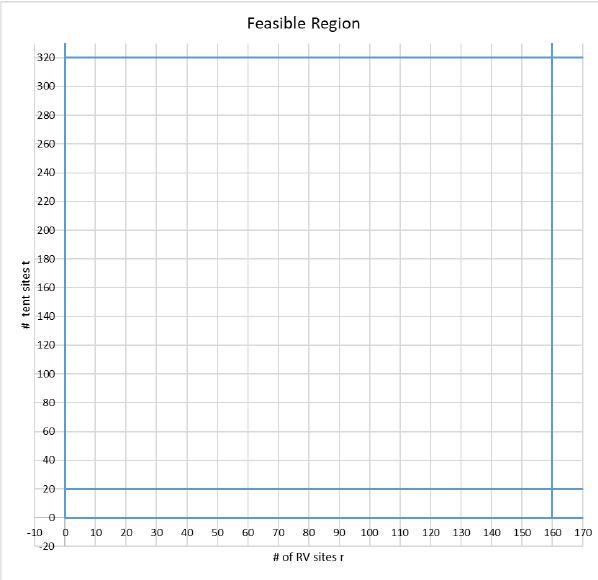
\includegraphics[scale = 0.5]{2022_07_05_5945264bba2a5f6ba667g-28}

Adding the remaining constraints yields this graph: Go ahead, shade the feasible region and identify all redundant constraints.

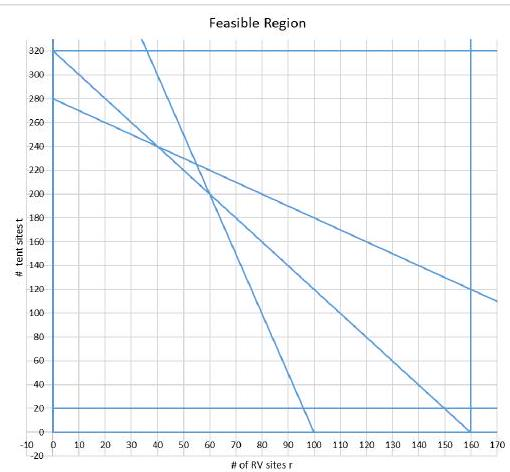
\includegraphics[scale = 0.5]{2022_07_05_5945264bba2a5f6ba667g-29}

All the points in the feasible region are possible solutions. Your job is to pick (one of) the best solutions. Note that there may not be a single best solution but rather several optimal solutions.

We have not yet used the objective function $P(r, t)=80 r+20 t$. Because we do not have a value for $P(r, t)$, so we will draw $P(r, t)$ for a few random values of $P(r, t)$ to get an idea of what it looks like. For $P(r, t)=1600,2400,3200$ we get the lines shown in the next picture. Note that they are all parallel, and that the lines corresponding to the larger value of $P(r, t)$ move to the top left. The direction of increase is just as we expected, to the top right.

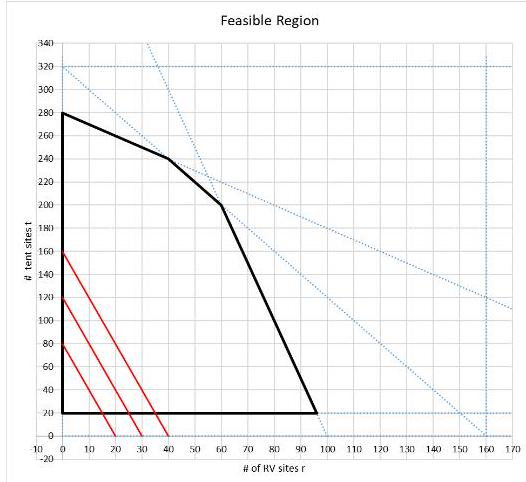
\includegraphics[scale = 0.5]{2022_07_05_5945264bba2a5f6ba667g-29(1)}

As you move the line for the $P(r, t)$ to the right you increase your profit. But you also have to stay in the feasible region. Convince yourself that one of two cases will occur: either a unique optimal solution will be found at a corner point, or infinitely many optimal solutions returning the same maximum value for $P(r, t)$ will be found along a section of the boundary of the feasible region that includes two corner points. Therefore, we need to compute the corner points, i.e. the intersections of the constraints, and move $P(r, t)$ as far to the right as possible without leaving the feasible region.

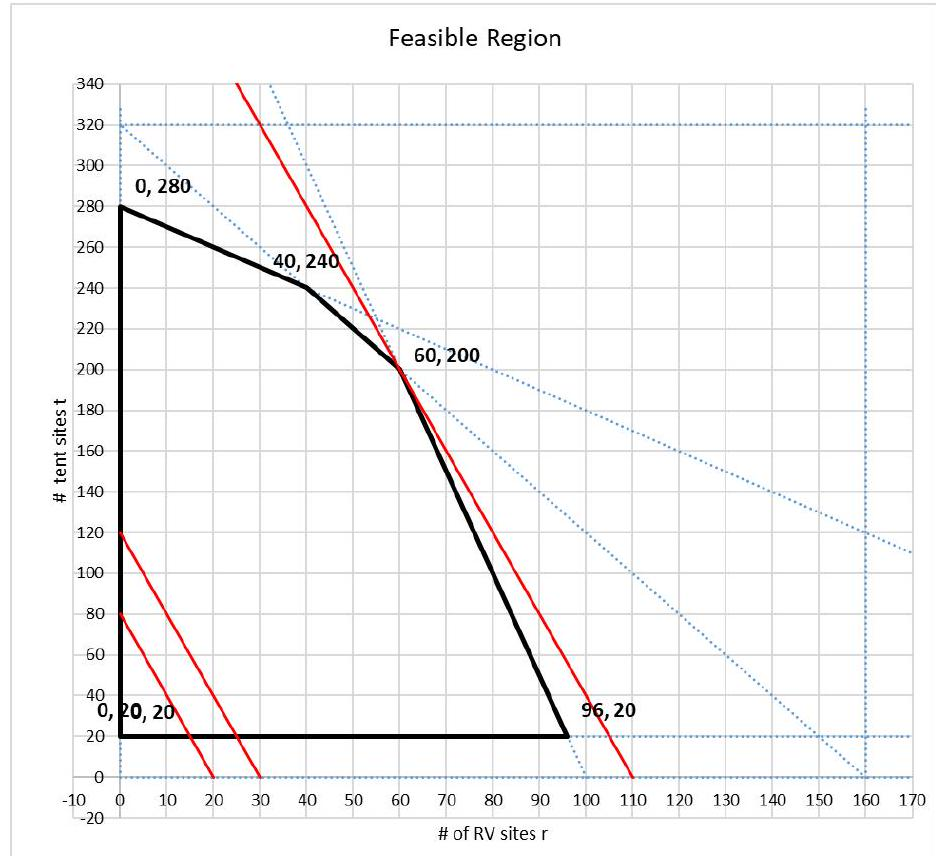
\includegraphics[scale = 0.5]{2022_07_05_5945264bba2a5f6ba667g-30}

From the picture above, you can see that the optimal solution will be at the intersection of the lines corresponding to constraints 1) and 5).
$$
r / 20+t / 40 \leq 8 \text { and } 1000 t+200 t \leq 100,000
$$
which is at the point $r=60, t=200$. (Now would be a good time to review how to solve systems of equations....). This gives us a profit $P(60,200)=60 \cdot \$ 80+200 \cdot \$ 20=\$ 8800$.

\subsection{Stating the Solution}
In OR, typically someone hires you to work your problem, and then expects you to give the answer in the context of the problem. You can't just say "the solution is at $r=60, t=200, P(r, t)=8800$ ". Give the answer like this:

"To maximize potential profit, the campground should have $60 \mathrm{RV}$ sites and 200 tent sites. In that case, the potential profit per day, assuming full occupancy, is $\$ 8800$. You are limited by the available land and budget available, not by available labor or any zoning rules. You will have to hire 65 hours of help per week (260 camping units at 15 minutes/week/unit)."

\subsection{Refinements to the graphical solution}
One "brute force" approach to the graphical solution method would be to compute all intersections of all constraints, check if that corner is in the feasible region, and then compute the objective function at those points. However, the number of intersections increases quadratically with the number of lines ( $\frac{\mathrm{n}(\mathrm{n}+1)}{2}$ for $n$ non-parallel lines), so this approach quickly gets out of hand. Instead, the idea is to start at an easy to find corner of the feasible region. Often, the origin works. From that point, check the adjacent feasible corner points and move to the "best". Continue until there is no more improvement. Here is what that would look like in our case:

We start at a simple corner. Usually, people use the origin, which is not on the feasible region here, so we start at $(0,20)$. Adjacent corners are $(0,280)$ and $(96,20)$ with $P(0,20)=400, P(0,280)=5600$, and $P(96,20)=8080$. $(96,20)$ is best, so we move there. Next, check the adjacent corner $(60,200)$. It gives $P(60,200)=8800$ which is an improvement, so move there. Check the next adjacent corner $(40,240)$ It gives $P(40,240)=8000$. This is worse, so $(60,200)$ is the optimal solution.\\

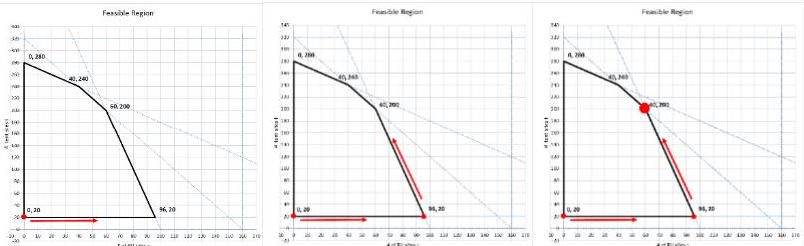
\includegraphics[scale = 0.5]{2022_07_05_5945264bba2a5f6ba667g-31}

There is of course a big problem with this approach. It relies on us having a graph of the feasible region and being able to see the adjacent feasible corner points. If you are dealing with a large number of constraints and variables, this is not possible. We therefor take the idea of looking at adjacent feasible corners and moving towards the one that gives the best value for the objective function, and translate it into an algebraic method.

\subsection{Solution Approach - Algebraic Simplex Method}
As these are only three variables, we could still draw the feasible region, now a solid bound by planes. However, we need an approach that works for any number of variables. The key to this method is the fact that an optimal solution will occur at a corner point of the feasible region. While the n-dimensional proof is beyond the scope of this class, this fact should be intuitively clear in the 2-d and 3-d cases.

We will first demonstrate the algebraic method on the two-variable problem (RV and tent only) and then solve the full problem.

\subsection{Corner points, interior corner points, slack variables}
We introduce slack variables to turn the inequalities into equalities. Basically, a slack variable lets you know how close you are to maxing out the constraint. In the current case, we have:

\begin{tabular}{ll}
Constraints &
Augmented constraints\\
1) $4 r+t \leq 320$ &
1) $2 r+t+s_{1}=320$\\
2) $5 r+t \leq 500$&
2) $5 r+t+s_{2}=500$\\
3) $r+t \leq 280$&
3) $r+t+s_{3}=280$\\
4) $t \geq 20$&
4) $\mathrm{t}-\mathrm{s}_{4}=20$\\
5) $r, t \geq 0$&
5) $r, t, s_{1}, s_{2}, s_{3}, s_{4} \geq 0$
\end{tabular}

A point is a corner point if it sits at the intersection of two or more constraints, i.e. if two or more slack variables are zero. A point is a feasible solution (i.e. inside the feasible region) if all slack variables are non-negative. A point is outside the feasible region if any slack variable is negative. We will from now on express each point as $\left(r, t, s_{1}, s_{2}, s_{3}, s_{4}\right)$. Given $r$ and $t$, one computes the values of the slack variables from the augmented constraints.

$\begin{array}{lllll}\text { Examples: } & r=100, t=20 \quad \rightarrow \quad(100,20,100,-20,140,0) & \text { outside the feasible region } \\ & r=10, t=30 \quad & \rightarrow & (10,30,270,420,240,10) & \text { inside feasible region } \\ r=150, t=20 & \rightarrow & (150,20,0,-270,110,0) & \text { corner outside feasible region }\end{array}$

\subsection{Initializing}
Because $(0,0)$ is not on the feasible region, we again start at $(r, t)=(0,20)$, which has the augmented form $(0,20,300,480,240,0)$. We are sitting on the intersection of the lines $r=0$ and $t=20$.

\subsection{The adjusted objective function}
Note: If the origin is a feasible corner point and you start at the origin, you can skip this step.

We are sitting on the intersection of the lines $r=0$ and $t=20$. To reach the next adjacent corner, we have to move along one of those lines, but which one? If we move along the line $r=0$, we move away from the line $t=20$, which is the same as saying we are increasing the corresponding slack, $s_{4}$. If we move along the line $t=20$, we increase $r$. We want to choose the direction of increase that gives us the fastest increase in $P$. The original objective function is $P(r, t)=80 r+20 t$, which does not let us see what happens if we increase $s_{4}$ We have to rewrite $P(r, t)$ in terms of $r$ and $s_{4}$.

Using equation 4) we get $t=20+s_{4}$, and thus $P\left(r, s_{4}\right)=80 r+20\left(20+s_{4}\right)=400+80 r+20 s_{4}$

\subsection{Determining which way to move}
We want to choose the direction of increase that gives us the fastest increase in P. The objective function is $P\left(r, s_{4}\right)=400+80 r+20 s_{4}$. Because the variable $r$ has the biggest coefficient, 80 , an increase in r should give the best return.

\subsection{Determining how far to move - the next corner}
We will leave $s_{4}$ at is current value, 0 , and increase $r$ as much as possible without leaving the feasible region, i.e. without having $t, s_{1}, s_{2}, s_{3}, s_{4}$ become negative.

\begin{enumerate}
  \item $2 r+t+s_{1}=320$\\
$s_{1}=320-20-2 r \geq 0$, so $r \leq 150$\\
$s_{2}=500-20-5 r \geq 0$, so $r \leq 96$
  \item $5 r+t+s_{2}=500$\\
$S_{3}=280-20-r \geq 0$, so $r \leq 240$
  \item $r+t+s_{3}=280$
  \item $t-S_{4}=20$\\
$t=20$
\end{enumerate}
So, $r$ can be increased to 96 .

\subsection{Augmented form of the next corner}
Using $r=96, s_{4}=0$, and substituting into the equations $1-4$, we have the augmented point $(96,20,108,0$, $164,0)$. Note that this is the same corner $(96,20)$ we used above.

\subsection{The adjusted objective function}
We are now sitting on the intersection of the lines $5 r+t+s_{2}=500$ and $t=20$. To reach the next adjacent corner, we have to move along one of those lines, which means either increasing $s_{2}$ or $s_{4}$. We have to rewrite $P(r, t)$ in terms of $s_{2}$ and $s_{4}$.

Using equations 2 and 4 , we find that $5 r=500-t-s_{2}$ and $t=20+s_{4}$, which yields $5 r=480-s_{4}-s_{2}$. Substituting into $P$ :

$P\left(s_{2}, s_{4}\right)=400+80 r+20 s_{4}=400+16\left(480-s_{4}-s_{2}\right)=20 s_{4}=8080+4 s_{4}-16 s_{2}$

Now we will repeat the above steps until the solution/objective function can no longer be improved upon.

\subsection{Determining which way to move}
Because the $\mathrm{S}_{4}$ has the only positive coefficient, this is the only direction that will yield an increase in $\mathrm{P}$.

\subsection{Determining how far to move - the next corner}
We will leave $s_{2}$ at is current value, 0 , and increase $s_{4}$ as much as possible without leaving the feasible region.

\begin{enumerate}
  \item $2 r+t+s_{1}=320 \quad s_{1}=320-t-2 r$
  \item $5 r+t+s_{2}=500$\\
$\mathrm{s}_{2}=500-\mathrm{t}-5 \mathrm{r}$
  \item $r+t+s_{3}=280$\\
$\mathrm{s}_{3}=280-\mathrm{t}-\mathrm{r}$
  \item $t-s_{4}=20$ $\mathrm{t}=20+\mathrm{s}_{4}$
\end{enumerate}
We use that $s_{2}=0$ and $t=20+s_{4}$. This gives the set of equations:

\begin{enumerate}
  \item $s_{1}=108-0.6 s_{4}$\\
$\geq 0$, so $\mathrm{s}_{4} \leq 96$\\
$\geq 0$, so $\mathrm{S}_{4} \leq 480$

  \item $r=96-0.2 s_{4}$\\
$\geq 0$, so $\mathrm{S}_{4} \leq 205$

  \item $\mathrm{s}_{3}=164-0.8 \mathrm{~s}_{4}$

  \item $t=20+s_{4}$

\end{enumerate}
$\geq 0$, so $\mathrm{s}_{4} \geq-20$ (as 20 is positive, this is true anyway) So $\mathrm{S}_{4}$ can be increase up to 180 .

\subsection{Augmented form of the next corner}
Using $s_{2}=0, s_{4}=180$, and substituting into the equations $1-4$, we have the augmented point $(60,200,0,0$, $20,180)$. Note that this is the second corner $(60,200)$ we used above.

\subsection{The adjusted objective function}
We again re-write the objective function, this time in terms of $s_{1}$ and $s_{2}$ : $P\left(s_{1}, s_{2}\right)=8080+4 s_{4}-16 s_{2}=8080+4\left(180-1.6 s_{1}\right)-16 s_{2}=8800-6.6 s_{1}-16 s_{2}$. Note that increasing either $s_{1}$ or $s_{2}$ will decrease the value of $P$, so we have reached the maximum. As $s_{1}$ and $s_{2}$ are non-negative, we can also see that the maximum for $P$ occurs when $s_{1}$ and $s_{2}$ are zero, at $P=8800$. Again, this is the same answer we arrived at earlier.

A nice side effect is that we can tell which constraints are holding us back, namely those associated with the zero slack variables $s_{1}$ and $s_{2} . s_{1}$ corresponds to the space limitations, and $s_{2}$ to the budget restrictions.

\subsection{Solving the full problem}
We are now ready to look at the original problem. We will assume you went to the bank and got a loan for $\$ 246,000$ to supplement your original budget. Here are the constraints again:

\begin{enumerate}
  \item Infrastructure takes up $20 \%$ of your site

  \item You can have $20 \mathrm{RV}$ s per acre, or

  \item You can have 40 tents per acre, or

  \item You can have 10 yurts per acre

  \item You have a budget of $\$ 346,000$. It costs you $\$ 1000$ to develop an RV site, $\$ 200$ for a tent site, and $\$ 8000$ for a yurt.

  \item Maintenance for the bath houses etc. is $15 \mathrm{~min} /$ week/camper unit, you can afford $70 \mathrm{hrs} /$ week in maintenance help

  \item Zoning ordinance requires you to have at least 20 tent sites

\end{enumerate}
\begin{tabular}{|l|l|l|}
\hline
Functional Constraints & $\underline{\text { Simplified Constraints }}$ & $\underline{\text { Augmented Constraints }}$ \\
\hline
$\mathrm{r} / 20+\mathrm{t} / 40+\mathrm{y} / 10 \leq 8$ & $2 \mathrm{r}+\mathrm{t}+4 \mathrm{y} \leq 320$ & $2 \mathrm{r}+\mathrm{t}+4 \mathrm{y}+\mathrm{s}_{1}=320$ \\
$1000 \mathrm{r}+200 \mathrm{t}+8000 \mathrm{y} \leq 346,000$ & $5 r+t+40 \mathrm{y} \leq 1730$ & $5 \mathrm{r}+\mathrm{t}+40 \mathrm{y}+\mathrm{s}_{2}=1750$ \\
$(\mathrm{r}+\mathrm{t}+\mathrm{y}) / 4 \leq 70$ & $\mathrm{r}+\mathrm{t}+\mathrm{y} \leq 280$ & $\mathrm{r}+\mathrm{t}+\mathrm{y}+\mathrm{s}_{3}=280$ \\
$\mathrm{t} \geq 20$ & $\mathrm{t} \geq 20$ & $\mathrm{t}-\mathrm{s}_{4}=20$ \\
\hline
\end{tabular}

\subsection{Non-negativity constraints:}
$r, t, y_{1}, s_{1}, s_{2}, s_{3}, s_{4} \geq 0$

\subsection{Objective function:}
Maximize $P(r, t, y)=80 r+20 t+200 y$

\subsection{Initializing}
Because $(0,0,0)$ is not on the feasible region, we start at $(r, t, y)=(0,20,0)$, which has the augmented form $(0,20,0,300,480,240,0)$. We are sitting on the intersection of the planes $r=0, t=20, y=0$. The augmented form of this corner is $(0,20,0,300,1710,260,0)$

\subsection{The adjusted objective function}
Rewriting $P$ as $P\left(r, y, s_{4}\right)$ gives: $P\left(P\left(r, y, s_{4}\right)=400+80 r+200 y+20 s_{4}\right.$

\subsection{Determining which way to move}
Looking at the coefficients of $r, y, s_{4}$ in the objective function, we find that we should increase $y$ and leave $r$ and $s_{4}=0$

\subsection{Determining how far to move - the next corner}
Using $r=0$ and $s_{4}=0$, the constraints become

$\begin{array}{lllll}t+4 y+s_{1}=320 & 4 y+s_{1}=300 & s_{1}=300-4 y & \geq 0 & \rightarrow y \leq 75 \\ t+40 y+s_{2}=1750 & 40 y+s_{2}=1730 & s_{2}=1730-40 y & \geq 0 & \rightarrow y \leq 42.75 \\ t+y+s_{3}=280 & y+s_{3}=260 & s_{3}=260-y & \geq 0 & \rightarrow y \leq 260\end{array}$

$t=20$

So, y can be increased up to $42.75$

\subsection{Augmented form of the next corner}
With $\mathrm{r}=0, \mathrm{~s}_{4}=0$, and $\mathrm{y}=42.75$, we find the new augmented corner to be $(0,20,42.75,129,0,217.25,0)$.

\subsection{The adjusted objective function}
We need to rewrite the objective function in terms of $r, s_{2}$, and $s_{4}$ :

$P\left(r, s_{2}, s_{4}\right)=8950+55 r+15 s_{4}-5 s_{2}$

The solution is not optimal yet, (there are still positive coefficients in the objective function), so we keep going.

\subsection{Determining which way to move}
We see that we should increase $r$ and leave $s_{2}$ and $s_{4}=0$.

Determining how far to move - the next corner

With $s_{2}$ and $s_{4}=0$, we have

$\begin{array}{llll}2 r+t+4 y+s_{1}=320 & 2 r+4 y+s_{1}=300 & s_{1}=129-1.5 r \geq 0 & \rightarrow r \leq 86 \\ 5 r+t+40 y=1750 & 5 r+40 y=1730 & 40 y=1710-5 r & \\ r+t+y+s_{3}=280 & r+y+s_{3}=260 & s_{3}=236.25-0.875 r \geq 0 & \rightarrow r \leq 342\end{array}$

$t=20$

So, y can be increased up to 86

\subsection{Augmented form of the next corner}
With $y=86, s_{2}=2$, and $s_{4}=0$ we find the new augmented corner to be $(86,20,32,0,0,142,0)$

\subsection{The adjusted objective function}
We need to rewrite the objective function in terms of $s_{1}, s_{2}$, and $s_{4}$ :

$P\left(s_{1}, s_{2}, s_{4}\right)=13680-36 \frac{2}{3} s_{1}-1 \frac{1}{3} s_{2}-18 s_{4}$

Note that now all variables have negative coefficients, so we cannot increase the value of P past 13680. The first, second, and fourth constraints are maxed out; we are limited in our ability to increase the profit by space, money, and zoning restrictions.

\subsection{ Stating the Solution }
To maximize potential profit, the campground should have 86 RV sites, 20 tent sites, and 32 yurts. This will take an initial investment of $\$ 346,000$. The potential profit per day, assuming full occupancy, is $\$ 13,680$. You are limited by the available land and budget available and the zoning law requiring 20 tent sites. You will have to hire $34.5$ hours of help per week (138 camping units at 15 minutes/week/unit)."

\subsection{Solution Approach - Using Excel}
Now that we know how the solution method works, we can use Excel to do the work for us. First, we must set up the work sheet. One way that works well is shown on the next page. The fields highlighted in green are necessary, the others serve to explain and label what we are doing.

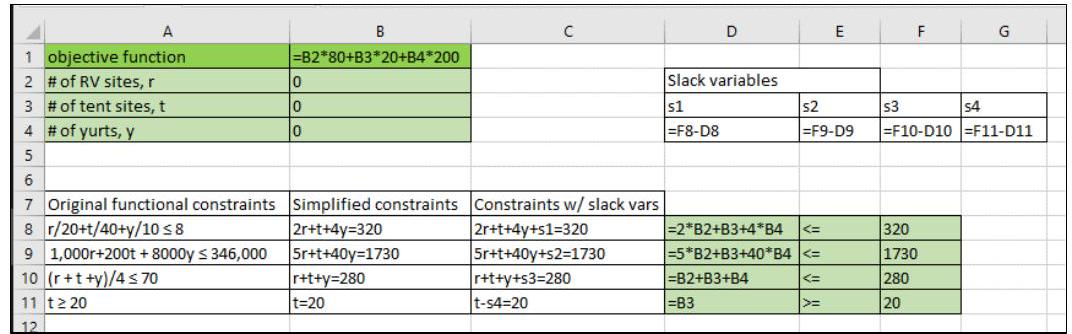
\includegraphics[scale = 0.5]{2022_07_05_5945264bba2a5f6ba667g-37}

Excel has a built-in Solver under the Data tab (if you don't see it, you have to add it in. Go to file/options/Add-ins/Manage Excel Add-ins/Solver Add-in). If you choose "show iteration results in the options tab, the solver will stop at each iteration and show you the corner/solution it has arrived found at that step. You will see that the solver goes through the same steps and corner points as we did when we worked the problem "by hand".

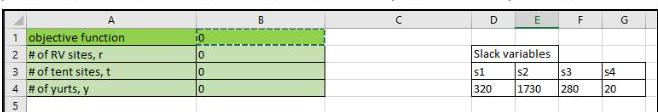
\includegraphics[scale = 0.5]{2022_07_05_5945264bba2a5f6ba667g-37-1}

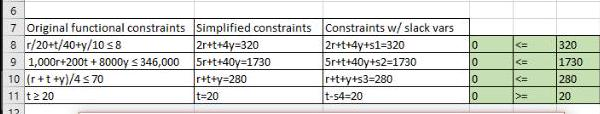
\includegraphics[scale = 0.5]{2022_07_05_5945264bba2a5f6ba667g-37-2}

$All Methods | GRG Nonlinear | Evolutionery |$

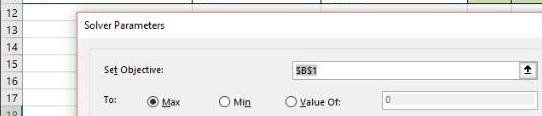
\includegraphics[scale = 0.5]{2022_07_05_5945264bba2a5f6ba667g-37(3)}

Constrainterecisioni. $\quad 0.000001 .$

- Automatic scaling

Whe Automatic scoling

Whow lteration results

Solving with integer Constraints

Solving with integer constraints

\begin{tabular}{l|l|l|}
18 & By Changing Variable Cells: & \$ \\
\hline
19 & SBS2:SBS4 &  \\
20 & Subject to the Constraints: & SDS11 = SFs11 \\
\hline
21 &  &  \\
\hline
\end{tabular}

$\square$ Ignoce integer constraints

By Changing Variable Cells:

$\mathrm{~ - ~ T ~ 2 ~}$

1

(2. $\quad$ Solving Limits

4

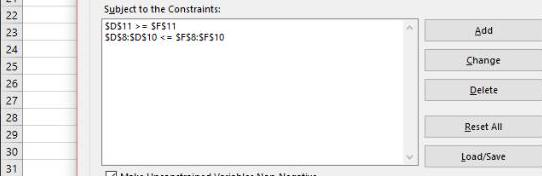
\includegraphics[scale = 0.5]{2022_07_05_5945264bba2a5f6ba667g-37(4)}

Subbject to the Constraints:

Max Iime |Seconds|:

Iterations:

Evolutionary and Integer Constraints:

Evolutionary and inteE

Lox subprobiems:

Mox Ecosible Solutions:

Options


\includegraphics[scale = 0.5]{2022_07_05_5945264bba2a5f6ba667g-37(5)}

\begin{itemize}
  \item 
\end{itemize}
$\square$ Make Unconstrained Variables Non-Negative

Select a Solvin\\
Method:

ORtions

Solving Method

Solving Method Select the GRG Nonlinear engine for Solver Problems that are smooth nonlinear. Select the\\
Simplex engine for linear Solver Problems, and select the Evolutionary engine for Solver problems that are non-smooth.

Help

Solve

Close
